
% !TEX TS-program = pdflatex
% !TEX encoding = UTF-8 Unicode

% This file is a template using the "beamer" package to create slides for a talk or presentation
% - Giving a talk on some subject.
% - The talk is between 15min and 45min long.
% - Style is ornate.

% MODIFIED by Jonathan Kew, 2008-07-06
% The header comments and encoding in this file were modified for inclusion with TeXworks.
% The content is otherwise unchanged from the original distributed with the beamer package.

\documentclass{beamer}
\newtheorem{proposition}{Proposition}


% Copyright 2004 by Till Tantau <tantau@users.sourceforge.net>.
%
% In principle, this file can be redistributed and/or modified under
% the terms of the GNU Public License, version 2.
%
% However, this file is supposed to be a template to be modified
% for your own needs. For this reason, if you use this file as a
% template and not specifically distribute it as part of a another
% package/program, I grant the extra permission to freely copy and
% modify this file as you see fit and even to delete this copyright
% notice. 


\mode<presentation>
{
  \usetheme{Warsaw}
  % or ...

  \setbeamercovered{transparent}
  % or whatever 
}


\usepackage[english]{babel}
% or whatever

\usepackage[utf8]{inputenc}
% or whatever
\usepackage{mathrsfs}  

\usepackage{times}
\usepackage{amsmath}
\usepackage[T1]{fontenc}
% Or whatever. Note that the encoding and the font should match. If T1
% does not look nice, try deleting the line with the fontenc.


\title[title] % (optional, use only with long paper titles)
{$\mathcal{U}$-Bootstrap percolation}

\author[Davy, Gjorgjevski, Pak] % (optional, use only with lots of authors)
{Leo Davy \and Martin Gjorgjevski \and Alexandre Pak}
% - Use the \inst{?} command only if the authors have different
%   affiliation.

\institute[ENS Lyon] % (optional, but mostly needed)
{
  ENS Lyon \\
  M2 Advanced Mathematics}
% - Use the \inst command only if there are several affiliations.
% - Keep it tildeple, no one is interested in your street address.

\date[Short Occasion] % (optional)
{March 2022}

\defbeamertemplate*{footline}{shadow theme}
{%
  \leavevmode%
  \hbox{\begin{beamercolorbox}[wd=.5\paperwidth,ht=2.5ex,dp=1.125ex,leftskip=.3cm plus1fil,rightskip=.3cm]{author in head/foot}%
    \usebeamerfont{author in head/foot}\insertframenumber\,/\,\inserttotalframenumber\hfill\insertshortauthor
  \end{beamercolorbox}%
  \begin{beamercolorbox}[wd=.5\paperwidth,ht=2.5ex,dp=1.125ex,leftskip=.3cm,rightskip=.3cm plus1fil]{title in head/foot}%
    \usebeamerfont{title in head/foot}\insertshorttitle%
  \end{beamercolorbox}}%
  \vskip0pt%
}
\setbeamertemplate{headline}
{%
  \leavevmode%
  \begin{beamercolorbox}[wd=.5\paperwidth,ht=2.5ex,dp=1.125ex]{section in head/foot}%
    \hbox to .5\paperwidth{\hfil\insertsectionhead\hfil}
  \end{beamercolorbox}%
  \begin{beamercolorbox}[wd=.5\paperwidth,ht=2.5ex,dp=1.125ex]{subsection in head/foot}%
    \hbox to .5\paperwidth{\hfil\insertsubsectionhead\hfil}
  \end{beamercolorbox}%
}

\setbeamertemplate{navigation symbols}{} 
\subject{Talks}
\begin{document}

\maketitle

\section{Introduction}
\begin{frame}{Update rules}
    
    \begin{itemize}
        \item An update rule is a finite set $X\subseteq\mathbb{Z}^2-\{0\}$
        \item An update family is a finite collection of update rules $\mathscr{U}=\{X\subseteq\mathbb{Z}^2-\{0\}\}$
    \end{itemize}
    
 
\begin{block}{}
   
 $\mathscr{U}$-Bootstrap percolation initialized at $A$ refers to the following process:

 \begin{itemize}
     \item $A_0=A$
     \item $A_{t+1}=A_t\cup \{x\in\mathbb{Z}^2: x+X\subseteq A_t \textit{ for some } X\in\mathscr{U}\}$
 \end{itemize}
 \end{block}
 
 \end{frame}
 \begin{frame}

 \begin{itemize}
 
 
     \item The set $A$ is known as the set of initially infected sites
     \item The closure of $A$ is defined as $[A]=\cup_{t\geq 0} A_t$
     \item The initialization is random i.e. each site (vertex)
     in $\mathbb{Z}^2$ is infected with probability $p$ independently from the other vertices
     \item The process is monotone i.e. if a site gets infected, it stays infected forever
     \item After the initialization, the process is deterministic in the sense that a site will get infected if and only if there is some rule $X$ in $\mathscr{U}$ such that $x+X$ is infected
 \end{itemize}
 


\end{frame}




\begin{frame}{Examples}

\begin{figure}[t]
    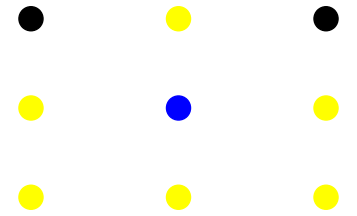
\includegraphics[width=0.18\textwidth]{rgospercrule.png}
    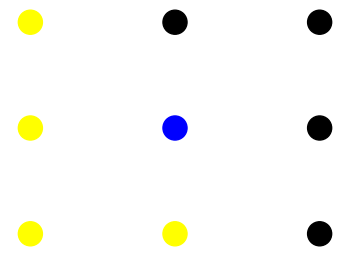
\includegraphics[width=0.15\textwidth]{rgspiralpercrule1.png}
    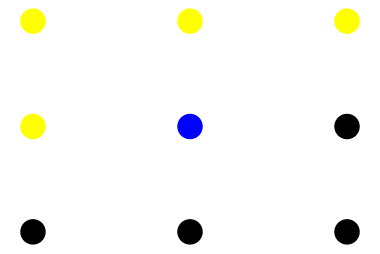
\includegraphics[width=0.17\textwidth]{rgspiralpercrule2.png}
    \caption{Oriented site, rules $U_1$ and $U_2$ for spiral model}
    \label{fig:mesh1}
\end{figure}
\begin{itemize}
    \item r-Neighbour models for r=1,2,3,4
    \item Oriented site $\mathscr{U}=\{(-1,1),(1,1)\}$
    \item Spiral $\mathscr{U}=\{U_1,U_2,U_3,U_4\}$, where 
    $U_1=\{(1,-1),(1,0),(1,1),(0,1)\}$
    \newline
    $U_2=\{(1,-1),(1,0),(-1,-1),(0,-1)\}
    $
    \newline
    $ U_3=-U_1, U_4=-U_2$
    \item Directed triangular bootstrap percolation 
    

\end{itemize}



\end{frame}

\begin{frame}{Stable directions, basic properties}
For a vector $u\in\mathbb{S}^1$, we define $
\mathbb{H}_u=\{x\in\mathbb{Z}^2|<x,u><0\}$.

\begin{block}{Definition}



Given an update family $\mathscr{U}$, a direction $u\in\mathbb{S}^1$ is
\begin{itemize}

    \item stable if $[\mathbb{H}_u]=\mathbb{H}_u$. The set of stable directions is denoted by $\mathscr{S}=\mathscr{S}{U}$
    \item strongly stable if $u\in int\mathscr{S}$
    \item unstable if it is not stable


\end{itemize}
\end{block}


\begin{itemize}
    \item Dichotomy $[\mathbb{H}_u]\in\{\mathbb{H}_u,\mathbb{Z}^2\}$
    \item $\mathscr{S}\subseteq\mathbb{S}^1$ is a set of stable directions for some update familit $\mathscr{U}$ if and only if it can be expressed as a union of closed intervals with rational endpoints\footnote{A direction $u\in\mathbb{S}^1$ is said to be rational if there is a point in the grid $\mathbb{Z}^2\cap\{\lambda u|\lambda\in\mathbb{R}\}$
    1}
    in $\mathbb{S}^1$
\end{itemize}



\end{frame}

\begin{frame}{Classification of $\mathscr{U}$-Bootstrap percolation}
$\mathscr{U}$-bootstrap percolation update families exhibit different properties based on their stable sets. Let $\mathscr{U}$ be an update family with a set of stable directions $\mathscr{S}$
\begin{block}

\begin{itemize}
    \item If there is a open semicircle $C$ such that $\mathscr{S}\cap C=\emptyset$ then $\mathscr{U}$ is said to be \textbf{supercritical}
    \item If every open semicircle $C$ intersects $\mathscr{S}$, but there is an open semicircle $C_0$ that doesn't intersect $int\mathscr{S}$ then $\mathscr{U}$ is said to be \textbf{critical}
    \item If every open semicircle $C$ intersects $int S$ then $\mathscr{U}$ is said to be \textbf{critical}
\end{itemize}

\end{block}

\end{frame}

\begin{frame}{Supercritical and critical families}
\begin{block}{Infection time of the origin}
The infection time of 0 is defined as $\tau_p=\inf\{t\in\mathbb{N}: 0 \in A_t\}$, given that $A_0=A$ is sampled according to a Bernoulli $p$ distribution
\end{block}

\begin{itemize}
    \item For supercritical families, $\tau_p=p^{-\Theta(1)}$ as $p\rightarrow 0$ with high probability
    \item For critical families, $\tau_p=\exp(p^{-\Theta(1)})$ as 
    $p\rightarrow 0$ with high probability
\end{itemize}

Corollary: For supercritical and critical families, $p_c=\inf\{p>0|P_p([A]=\mathbb{Z}^2)=1\}=0$ i.e. for any $p>0$ we have percolation.
\newline
However, for subcritical families the situation is different.

    
\end{frame}


\begin{frame}{$d_u^\theta$ measures directions that are difficult to infect}
	\begin{block}{Critical densities with conic boundary conditions}
		For $u\in \mathbb{S}^1$ and $\theta\in[-\pi, \pi]$
		$$d_u^\theta := \inf\left\{q\in[0,1], \sum_n n\mathbb{P}_q(0\not\in [(A\cup V_{u,u+\theta})\cap B_n]) < \infty\right\}$$
	\end{block}
	Morally, the critical probability with infection of $V_{u,u+\theta} = \mathbb{H}_u \cap \mathbb{H}_{u+\theta}$. 
	\begin{itemize}
		\item The summand decays slowly in $n$ when it is hard to infect the origin using only infections at distance less than $n$. So, when it is hard to infect 0,  $d_u^\theta$ is large\footnote{non zero...}.
		\item When $\theta \sim \pm \pi$, few sites are infected, so it is easy for the origin not to be infected, the summand can be large. Hence, $d_u^\theta$ decreases when $\theta\to 0$
		\item $d_u^\pm := \lim_{\theta \to 0^\pm} d_u^\theta$ can be large when a small number of infections is not enough to infect the origin, even with a whole half plane infected !. 
	\end{itemize}
\end{frame}

\begin{frame}
	\begin{theorem}
		For any $\mathcal{U}$-bootstrap percolation model, its critical probability
		\begin{equation*}
			\tilde q_c = \inf\{q\in[0,1], \sum_n n\mathbb{P}_q(0\not\in [A\cap B_n]) < \infty\}
		\end{equation*}
		is equal to the maximal value of its critical density function
		\begin{equation*}
			d_u = \max_{0^\pm} \inf\{q\in[0,1], \sum_n n\mathbb{P}_q(0\not\in[(A\cup V_{u, u + 0^\pm})\cap B_n] < \infty\}
		\end{equation*}
		for $u$ in any semicircle $C$, i.e.,
		\begin{equation*}
			\tilde q_c = \inf_{C\in \mathcal{C}} \sup_{u\in C} d_u.
		\end{equation*}

	\end{theorem}
\end{frame}

\begin{frame}
	Let's denote $E_{u, \theta} = \{0\not\in [(A\cup V_{u, u+\theta})\cap B_n]\}$. Then,
	\begin{equation*}
		E_{u, \pm\pi} = \{ 0 \not\in [A\cap B_n]\} \supset E_{u, \theta}
	\end{equation*}
	which gives that the following holds for any $u$
	\begin{equation*}
		\tilde q_c \geq \sup_\theta \sup_u d_u^\theta \geq \limsup_{\theta\to 0} \sup_u d_u^\theta = \sup_u d_u.
	\end{equation*}
	The theorem states that all those quantities are equal. 
	\begin{block}{Meaning of the theorem}
		The difficulty of the model is as hard as its most difficult direction. In this direction, infecting a half plane doesn't affect the infection of the origin.
	\end{block}
\end{frame}

\begin{frame}{Proving $\sup d_u \geq \tilde q_c$}
	The goal is to show, that for any $q'>\sup d_u$ it holds that
	\begin{equation*}
		\sum_n n \mathbb{P}_{q'}(0\not\in[A\cap B_n]) < \infty.
	\end{equation*}
	The idea is to show that, at $q'$, the origin is infected most of the time.
	\begin{block}{2-step percolation : $q' = \sup d_u + \varepsilon$}
		\begin{enumerate}
			\item Infect sites with probability $\varepsilon$ to find some structures
			\item Infecting new sites with probability $q$ allows structures to grow
		\end{enumerate}
	\end{block}
\end{frame}

\begin{frame}{Some details on the proof}
	\begin{itemize}
		\item The structures that grow are droplets, with sides $(u_i)_{i=1}^n$ depending on $\sup d_u$.
		\item In the second percolation, droplets of size $L$ grow into droplets of size $\geq (1+\delta)L$, for some $\delta > 0$.
		\item The proof can be done in any semi-circle, so we can get $\tilde q_c = \inf_{C\in\mathcal{C}}\sup_{u\in C} d_u$
		\item The proof contains that $\forall q> \sup d_u$, there exists a constant $c(q)>0$ such that
			\begin{equation*}
				\theta_n(q) \leq e^{-c(q)n}
			\end{equation*}
	\end{itemize}
\end{frame}

\begin{frame}{Applying the theorem}
	\begin{theorem}
		For any update rules $\mathcal{U}$,
		\begin{equation*}
			q_c \leq \tilde q_c = \sup_{u\in\mathbb{S}^1} d_u = \inf_{C\in\mathcal{C}} \sup_{u\in C} d_u.
		\end{equation*}
		In particular, if $\mathcal{U}$ is not subcritical, then $\tilde q_c = q_c = 0$ 
	\end{theorem}
	So, having knowledge on $u\mapsto d_u$ allows to upper bound $q_c$...
	\begin{block}{Proposition : (It's harder for submodels to infect)}
		For any sub-collection of rules $\mathcal{U}'\subset \mathcal{U}$
		\begin{equation*}
			q_c(\mathcal{U}) \leq \tilde q_c (\mathcal{U}) \leq \inf_C \sup_{u\in C} d_u(\mathcal{U'})
		\end{equation*}
	\end{block}
	... and it is not even necessary to know the critical density for the whole set of rules to get such bounds.
\end{frame}

\begin{frame}{First level bound}
	\begin{block}{$DTBP$ : Directed Triangular Bootstrap Percolation}
		Let $\mathcal{U}' = \{(-1, -1), (0,1)\}$, one of the rules of DTBP, then
		\begin{equation*}
			q_c(DTBP) \leq \tilde q_c(DTBP) \leq \inf_{C\in\mathcal{C}} \sup_{u\in C} d_u(\mathcal{U}').
		\end{equation*}
		Applying a general formula for one rule families (using OP) gives $q_c(DTBP) \leq 0.245...$\footnote{Previous known bound was 0.312}
	\end{block}
\end{frame}

\begin{frame}{Second level bound}
	However, knowing one rule subfamilies is not enough.
	\begin{block}{Spiral}
		For spiral, it is possible to compute $d_u$ for all pairs of rules, such that the difficulty on pairs is the same as the difficulty of some Bidirectional OP :
		\begin{equation*}
			q_c(Spiral) \leq \tilde q_c(Spiral) \leq 1 - p_c^{OP}.
		\end{equation*}
		And the result is tight.
	\end{block}

\end{frame}



\end{document}